\section{Introduction}

% context
The Sand Motor (or Sand Engine) is an innovative solution to
counteract the anticipated coastal recession due to sea level rise
\citep{Stive2013}. The Sand Motor is a 21 $\mathrm{Mm^3}$ mega
nourishment along the Dutch coast that is constructed well above storm
surge level and therefore largely shaped by wind. While the Sand Motor
accommodates fetches up to 1.0 km and is permanently exposed to wind,
the dry surface area is remarkably stable \citep{Hoonhout2017a}. An
armor layer consisting of shells, pebbles and cobbles prevent erosion
by wind and thus limit the sediment availability \citep[following the
definition of][]{Kocurek1999}. Consequently, the aeolian sediment
transport rates at the Sand Motor are limited to approximately 35\% of
the wind transport capacity \citep{Hoonhout2017a} making the Sand
Motor an availability-limited coastal system.

% what has been done?
In an availability-limited coastal system, not the wind transport
capacity, but the sediment availability governs the sediment supply
towards the dunes \citep{Houser2013}. Sediment availability can be
limited by various bed surface properties, like shells, salt crusts,
moisture and vegetation. Studies on the influence of bed surface
properties on aeolian sediment availability and transport started as
wind tunnel experiments \citep[e.g.][]{Belly1964, Howard1977,
  Dyer1986, Gillette1989}. These studies typically determine an
adapted threshold velocity that relates the theoretical wind transport
capacity to a measured sediment transport capacity
\citep{Bagnold1937b}. In the field, the influence of different bed
surface properties on sediment availability cannot easily be
distinguished and the sediment availability is often presented
spatially aggregated \citep{Jackson1998, Arens2001, Wiggs2004}. The
concept of critical fetch is a widely used approach for spatial
aggregation of sediment supply \citep[e.g.][]{Jackson1999,
  DavidsonArnott2005, DavidsonArnott2008, Bauer2009}. The critical
fetch is the distance over which the saltation cascade develops and
aeolian sediment transport becomes saturated \citep{Bauer2002}. Since
the saltation cascade develops slower when sediment is scarce, the
critical fetch is inversely proportional to the sediment supply
\citep{DelgadoFernandez2010}.

% what is needed?
Expressing the sediment supply in terms of critical fetch assumes that
saturated transport is reached if the available fetch is
sufficient. \citet{Hoonhout2017a} showed that sediment supply can be
severely limited even with fetches as large as at the Sand
Motor. Consequently, critical fetches may become very large or even
undefined and the definition and interpretation of the critical fetch
impractical \citep{Lynch2016, deVries2014b}. Moreover, significant
spatial variations in sediment supply were found in the Sand Motor
region that challenges the spatial aggregation of sediment
availability. Alternatively, aeolian sediment transport is expressed
in terms of local sediment availability without the need for spatial
aggregation \citep{deVries2014a, Hoonhout2016}. Such approach would
require detailed measurements on spatiotemporal variations in aeolian
sediment availability.

% what did we do?
This paper presents detailed measurements of aeolian sediment
transport rates from the Sand Motor during a six week field campaign
in the fall of 2014. Spatial differences in sediment transport rates
reveal the main erosion and deposition areas of aeolian
sediment. Temporal variations in aeolian sediment transport are still
expected to be correlated with the wind speed, but spatial variations
are expected to be correlated with local variations in sediment
availability. Understanding local sediment availability ultimately
helps improving gross aeolian sediment transport estimates in
availability-limited coastal systems.

\section{Field Site}
\label{sec:fieldsite2}

The Sand Motor mega nourishment was constructed in 2011 along the
Delfland coast in The Netherlands \citep[Figure
\ref{fig:fieldsite2},][]{Stive2013}.  The Delfland coast was originally
characterized by an alongshore uniform profile with an average dune
height of 13 m, a dune foot at about 5 m+MSL and a beach slope of
about 1:40.

The Sand Motor is constructed as a 21 $\mathrm{Mm^3}$ hook-shaped
peninsula that initially protruded about 1 km into the sea and
stretched over approximately 2 km alongshore. The original crest
height of the Sand Motor was on average about 5 m+MSL and locally 7
m+MSL; both are well above common surge level. Consequently, a
significant part of the Sand Motor is uniquely shaped by aeolian
processes that redistribute significant amounts of sediments within
the Sand Motor region \citep{Hoonhout2017a}.

\begin{figure}
  \centering
  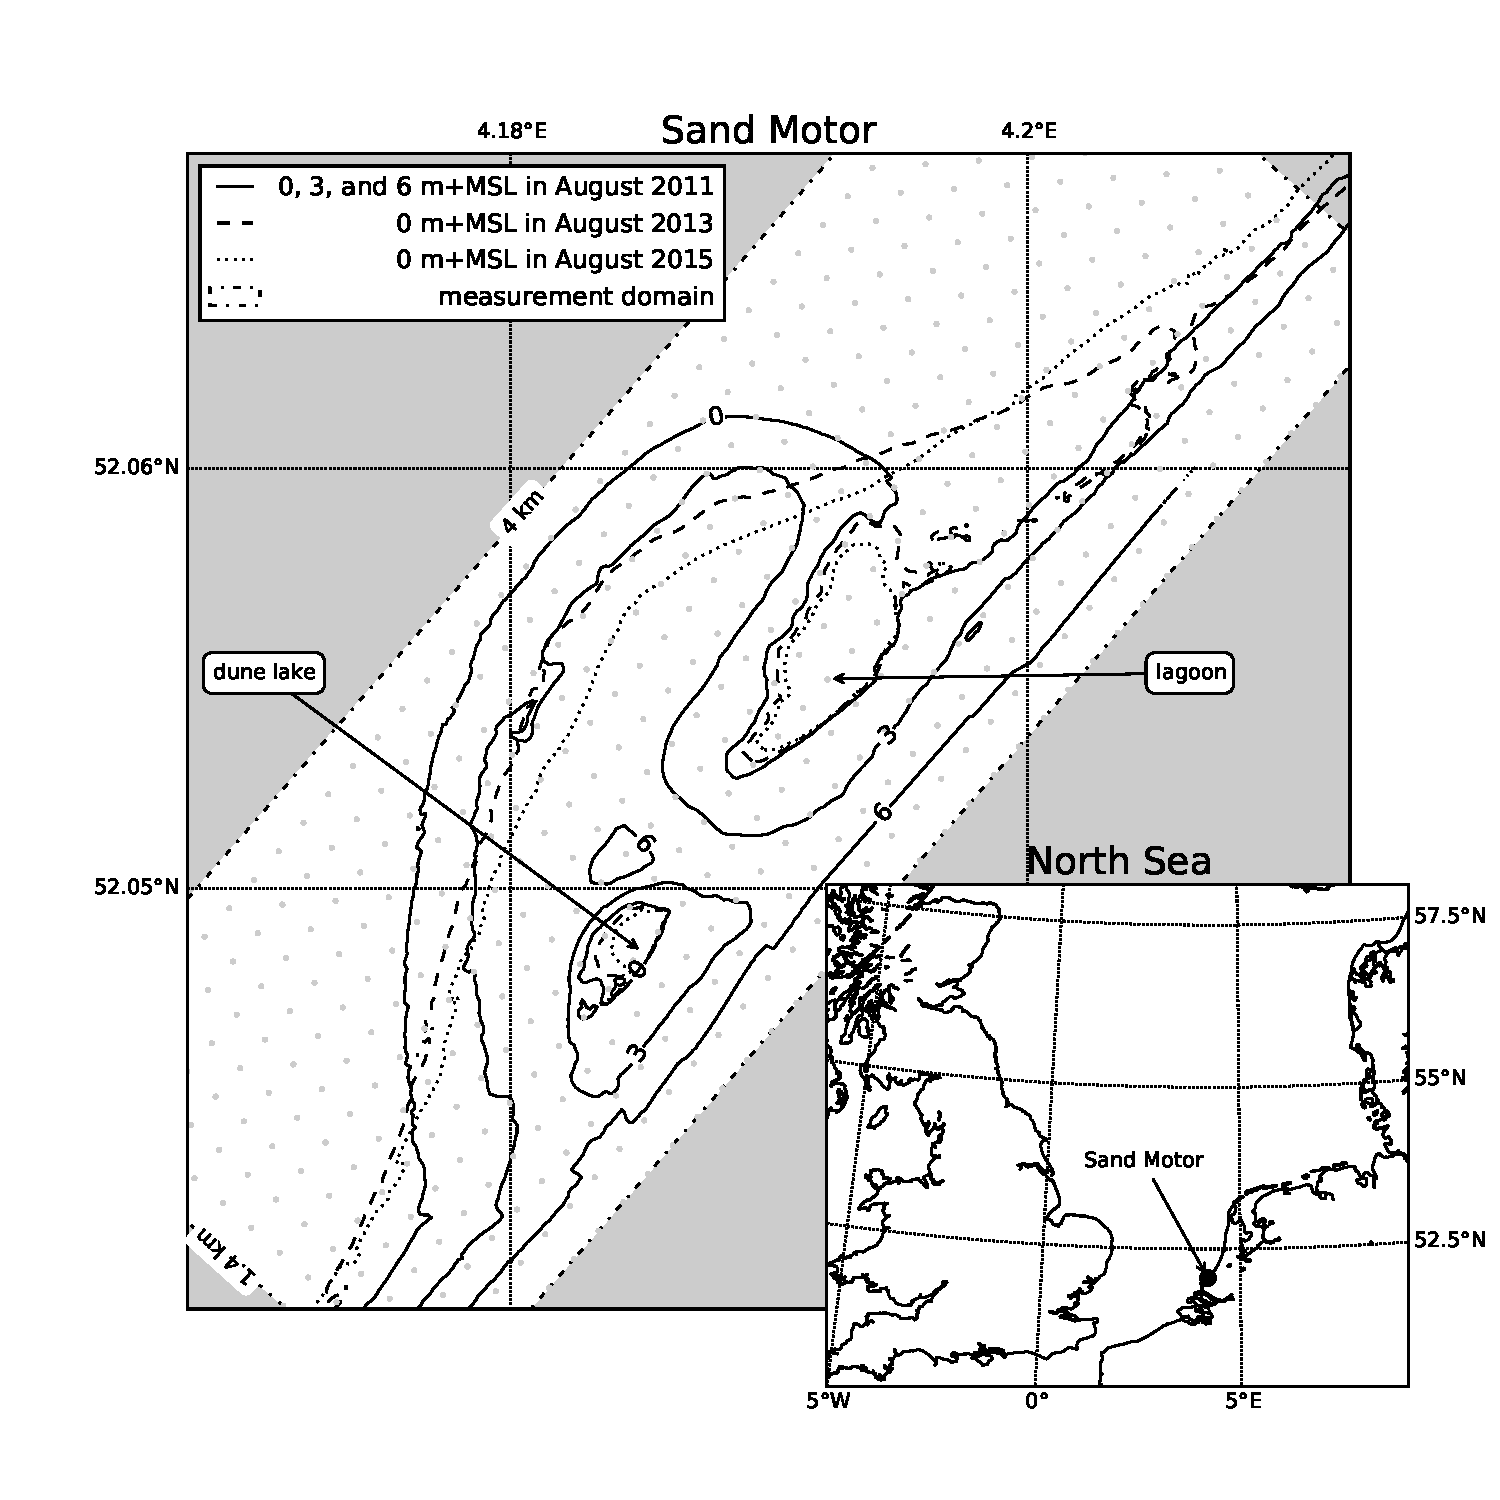
\includegraphics[width=\columnwidth]{../Figures/location_and_evolution}
  \caption{Location, orientation, appearance and evolution of the Sand
    Motor between construction 2011 and 2015. The box indicates the
    measurement domain used in the remainder of this paper. A 100 x
    100 m grid aligned with the measurement domain is plotted in gray
    as reference.}
  \label{fig:fieldsite2}
\end{figure}

Sand used for construction of the Sand Motor is medium sand with a
median diameter of about 350 $\mu \mathrm{m}$. The sand is obtained
from an offshore borrowing pit in the North Sea and contains many
shells and some pebbles, cobbles and other non-erodible material.

The predominant wind direction is south to southwest. Storms have a
tendency to be oriented either southwest or northwest. Also the
sediment transport potential ($\Psi$), defined as:

\begin{equation}
  \label{eq:transport_potential}
  \Psi \propto \int u^3 \mathrm{d}t
\end{equation}

\noindent in which $u$ is the wind speed, is predominantly
southwesterly or northwesterly oriented. The northwesterly storms are
generally accompanied with significant surges as the North Sea is
virtually unbounded in northwesterly direction (Figure
\ref{fig:fieldsite2}b).

The contour of the Sand Motor changed significantly in the four years
after construction. Tidal forces diffuse about 1 $\mathrm{Mm^3}$ per
year along the coast \citep{deSchipper2016}. Four years after
construction, the peninsula protrudes about 800 m into the sea and
stretches over 4 km alongshore (Figure \ref{fig:fieldsite2}).

%The tidal channel that connects the lagoon to the sea elongated and
%started to meander. Consequently, the 2 m tidal range that is present
%at the outer contour of the Sand Motor is damped over time to
%approximately 20 cm in the lagoon \citep{deVries2015}. At the closed
%end of the lagoon the tidal currents are therefore
%negligible. Consequently, morphological change in this area can be
%associated with aeolian sediment transport as is the morphological
%change in the dune lake.  The lagoon and dune lake therefore act as
%large sediment traps for aeolian sediment.

The Sand Motor provides a unique opportunity to perform measurements
on spatial variations in aeolian sediment availability and transport.
It accommodates vast and armored beaches next to dynamic intertidal
beaches of varying width, while limitations in fetch are negligible.

\section{Methodology}

Sediment transport measurements were performed to investigate the role
of the southern intertidal beaches as supplier of aeolian sediment in
the Sand Motor region \citep{Hoonhout2017a}. The change in sediment
transport in downwind direction (spatial gradient) was measured along
cross-shore transects running from the water line until the dry beach
at approximately 5 m+MSL. Spatial gradients in saltation transport are
positive in areas with net erosion and negative in areas with net
deposition of sediment. The measurements were performed
during the six week field campaign \textsc{MegaPEX} (Mega Perturbation
EXperiment) from September 17, 2014 until October 23, 2014.

\subsection{Equipment}

\begin{figure}
 \centering
  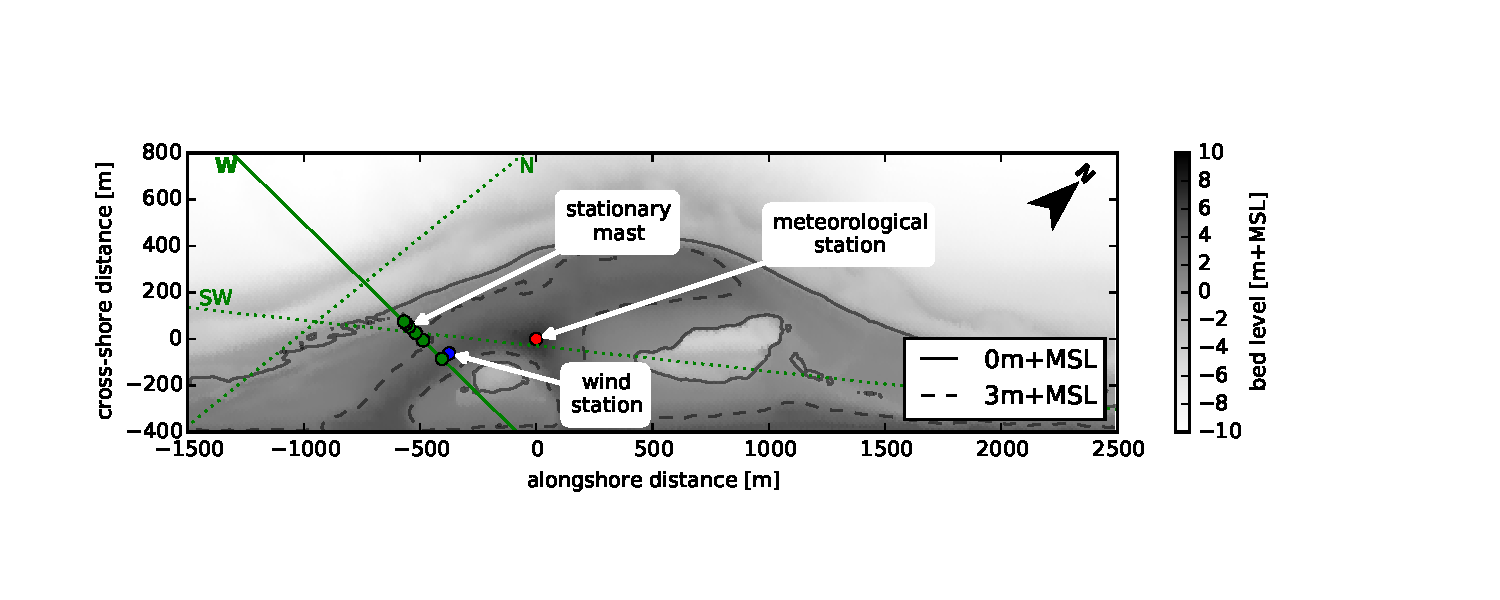
\includegraphics[width=\columnwidth]{../Figures/overview}
  \caption{Overview of measurement transects N, W, and SW and
    locations during the \textsc{MegaPEX} field campaign.}
  \label{fig:overview}
\end{figure}

\begin{figure}
 \centering
  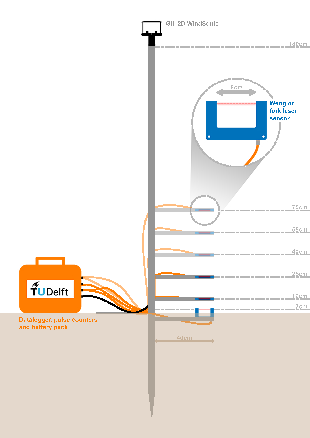
\includegraphics[width=\columnwidth]{../Figures/mast_small}
  \caption{Mast with 6 Wenglor fork laser sensors and a Gill 2D
    WindSonic ultrasonic wind speed and direction sensor viewed in
    direction of the wind. The top 3 laser sensors are optional.}
  \label{fig:mast}
\end{figure}

The measurement set-up consists of 8 masts with battery power and data
loggers. Each mast was equipped with at least three Wenglor fork laser
sensors (P/N: YH08PCT8) for saltation measurements at 3, 10 and 25 cm
above the bed (Figure \ref{fig:mast}). An additional three laser
sensors were added to the most landward mast at 40, 55 and 70 cm above
the bed to estimate the amount of particles bypassing the lower three
sensors. Other masts could be equipped with three additional laser
sensors as well. All except the lowest sensor were placed horizontally
with the arms directed towards the wind as to minimize the disturbance
of the wind field. The lowest sensor was placed vertically with the
arms directed upwards, and partially buried as to further minimize the
disturbance of the wind field. The Wenglor fork laser sensors register
passing particles of $50 ~ \mu \mathrm{m}$ and larger with a frequency
of 10 kHz using a laser beam of 0.6 mm. As the particle count is
linearly related to the sediment flux \citep{Hugenholtz2011}, both are
used indiscriminately in this study. The particle count is accumulated
by a HOBO pulse counter (P/N: S-UCC-M001). A HOBO Energy data logger
(P/N: H22-001) logged all sensors, including the pulse counters, at 1
Hz. In addition, three masts were equipped with a Gill 2D WindSonic
ultrasonic wind speed and direction sensor (P/N: 1405-PK-040) at a
height of 180 cm above the bed.

The masts can be rotated, but are not self-rotating to the wind as the
masts were relocated depending on the wind direction.  One stationary
mast was present during almost the entire field campaign (Figure
\ref{fig:overview}).

A separate Eijkelkamp wind station with three cup anemometers (P/N:
16.98.31) at heights 50, 100 and 180 cm and a wind vane (P/N:
16.98.34) at height 180 cm was present at a stationary location at the
high beach for the entire duration of the field campaign. A Campbell
Scientific meteorological station was present at the heart of the Sand
Motor providing measurements on precipitation, humidity, solar
radiation and wind speed and direction (Figure \ref{fig:overview}).

Qualitative small scale measurements on bed level change were
performed by pressing erosion pins (nails) in the beach with falling
tide. The erosion pins were placed along a cross-shore transect and
about 10 cm apart with their heads flush to the bed. The erosion
around the pins was measured manually with a ruler at the onset of
flood.

Daily topographic surveys are performed along cross-shore transects
using a Leica Viva GS10 RTG-GPS receiver. Offshore water levels and
wave heights are obtained from gauges at the permanent offshore
Europlatform.

\subsection{Deployments}

The measurement masts were deployed continuously during the field
campaign, but have been relocated according to the governing wind
direction. An overview of the measurement locations is given in Figure
\ref{fig:overview}. 

A single measurement transect consists of at least four masts: two in
the intertidal beach area in order to capture the entrainment rate
from the assumed sediment source region, one above the high water mark
to capture the sediment flux from the intertidal beach area onto the
dry upper beach and one higher up the beach to capture any additional
sediment supply from the dry beach itself. 

Table \ref{tab:deployments} lists the partitioning of the field
campaign in 10 deployments with constant location and orientation of
the measurement equipment. Most deployments were located along the
westerly transect at the southern flank of the Sand Motor (Figure
\ref{fig:overview}). Deployments DN02a and DN06a were aligned along
alternative transects concurrent with deployments DN02b and DN06b
respectively. During deployment DN11 all masts were clustered at high
grounds as to provide a safe buffer from the expected surge during the
storm event of October 23. Consequently, no transport gradients were
measured during deployment DN11.

\begin{table}[h]
  \centering
  \caption{Deployments of measurement masts during the \textsc{MegaPEX} field
    campaign. Maximum measured wind speeds are in parentheses.}
  \label{tab:deployments}
  \begin{tabular}[h]{lrrrrrrr}
    \hline
               & wind       &  wind      & laser      &   transect &   duration & sensors &     well \\
               & speed      & direction  & direction  &            &            &      &     oriented* \\
               &      [m/s] &     [$^o$] &     [$^o$] &            &        [h] &     [-] &       [\%] \\
    \hline
    DN02a      &     3 (10) &        358 &        262 &          W &         22 &       3 &          0 \\
    DN02b      &     3 (10) &        359 &        360 &          N &         22 &       3 &        100 \\
    DN04       &     5 (13) &        343 &        360 &          W &         42 &       3 &         92 \\
    DN05       &     3 (15) &        196 &        270 &          W &        312 &       3 &         40 \\
    DN06a      &     5 (17) &        166 &        225 &         SW &        170 &       3 &         55 \\
    DN06b      &     5 (17) &        180 &        225 &          W &        170 &       3 &         77 \\
    DN08       &     5 (16) &        199 &        225 &          W &        160 &       6 &         89 \\
    DN09       &     9 (21) &        240 &        270 &          W &         32 &       6 &         87 \\
    DN10       &    15 (22) &        301 &        315 &          W &          9 &       6 &        100 \\
    DN11       &    10 (24) &        322 &        315 &          - &         25 &       6 &         44 \\
    \hline
  \end{tabular}

  \footnotesize{
    \begin{enumerate}[{*}]
    \item The last column indicates the percentage of time in which
      the laser sensors were well oriented with respect to the wind.
      Raw data from all deployments is published as \citet{megapex}.
      DN01 is omitted from this list as it involved a test run of the
      equipment only. DN02a is listed only for convenience when
      interpreting the published dataset. DN02b and DN06b were
      originally named DN03 and DN07 respectively and can be found by
      these names only in the published dataset.
    \end{enumerate}}
\end{table}

\subsection{Data analysis}

Particle count time series obtained from individual Wenglor laser
sensors are summed up
\begin{enumerate}
\item per mast, to obtain \emph{per-mast} particle count time series
  for each measurement mast, and
\item over all masts, to obtain \emph{overall} particle count time
  series over all measurement masts.
\end{enumerate}
The per-mast particle counts are totaled rather than averaged, and
therefore not corrected for the number of Wenglor laser sensors per
mast. All masts deployed simultaneously in a single transect were
equipped with an equal number of sensors. Only the most landward mast
in the westerly transect was permanently equipped with six
sensors. However, the upper three sensors of the latter mast
registered negligible particle counts. Averaging would result in
approximately halving the per-mast particle counts. The halving of the
particle count does not reflect any physical behavior and is therefore
averted. Particle count time series are interchangeably referred to as
particle count rates as the measurement interval was 1 Hz.

The overall particle count time series are used for comparison with
the governing wind speed. For comparison with the wind direction
per-mast particle count time series are discretized in bins according
to the governing wind direction and subsequently summed over
time. Also for comparison with water and bed levels, the per-mast
particle count time series are discretized in bins and summed over
time. Discretization is then done according to the global water level
and local bed level at the measurement location.

Horizontal gradients in particle counts are computed from the per-mast
particle count time series and the distance between the measurement
masts. Vertical distributions in particle counts are computed from the
per-sensor particle count time series for each measurement mast.

Particle counts are converted into sediment fluxes following
\citet{Barchyn2014}:

\begin{equation}
  q_{\mathrm{wenglor}} = n_{\mathrm{wenglor}} \left( 
    \frac{6 \cdot \gamma}{\rho \pi D^3} \cdot l_{\mathrm{fork}} \cdot \left(
      l_{\mathrm{laser}} + D \right) \right)^{-1}
\end{equation}

\noindent with $\rho = 2650$ $\mathrm{kg/m^3}$,
$l_{\mathrm{fork}} = 8 \cdot 10^{-2}$ m,
$l_{\mathrm{laser}} = 6 \cdot 10^{-4}$ m, $D = 335$ $\mathrm{\mu m}$
and $\gamma = 1$.

Variations in wind direction of more than $45^o$ resulted in
adjustment of the orientation of the Wenglor fork laser
sensors. Particle counts with a discrepancy between wind direction and
laser orientation ($\Delta \theta_u$) of more than $60^o$ are
considered not well oriented and are discarded from the presented
analysis. Other particle counts ($n_{\mathrm{pc}}$) are corrected for
orientation inaccuracies ($\hat{n}_{\mathrm{pc}}$) using the basic
geometric correction:

\begin{equation}
  \hat{n}_{\mathrm{pc}} = \frac{n_{\mathrm{pc}}}{\cos(\Delta \theta_u)}
\end{equation}

Periods without significant particle counts are not discarded from the
analysis, except for the determination of the average wind direction
as the wind direction tends to show random behavior for low wind
conditions. The last column in Table \ref{tab:deployments} states the
percentage of time in the laser sensors were well oriented with
respect to the wind direction.

\section{Results}

\begin{figure}
 \centering
  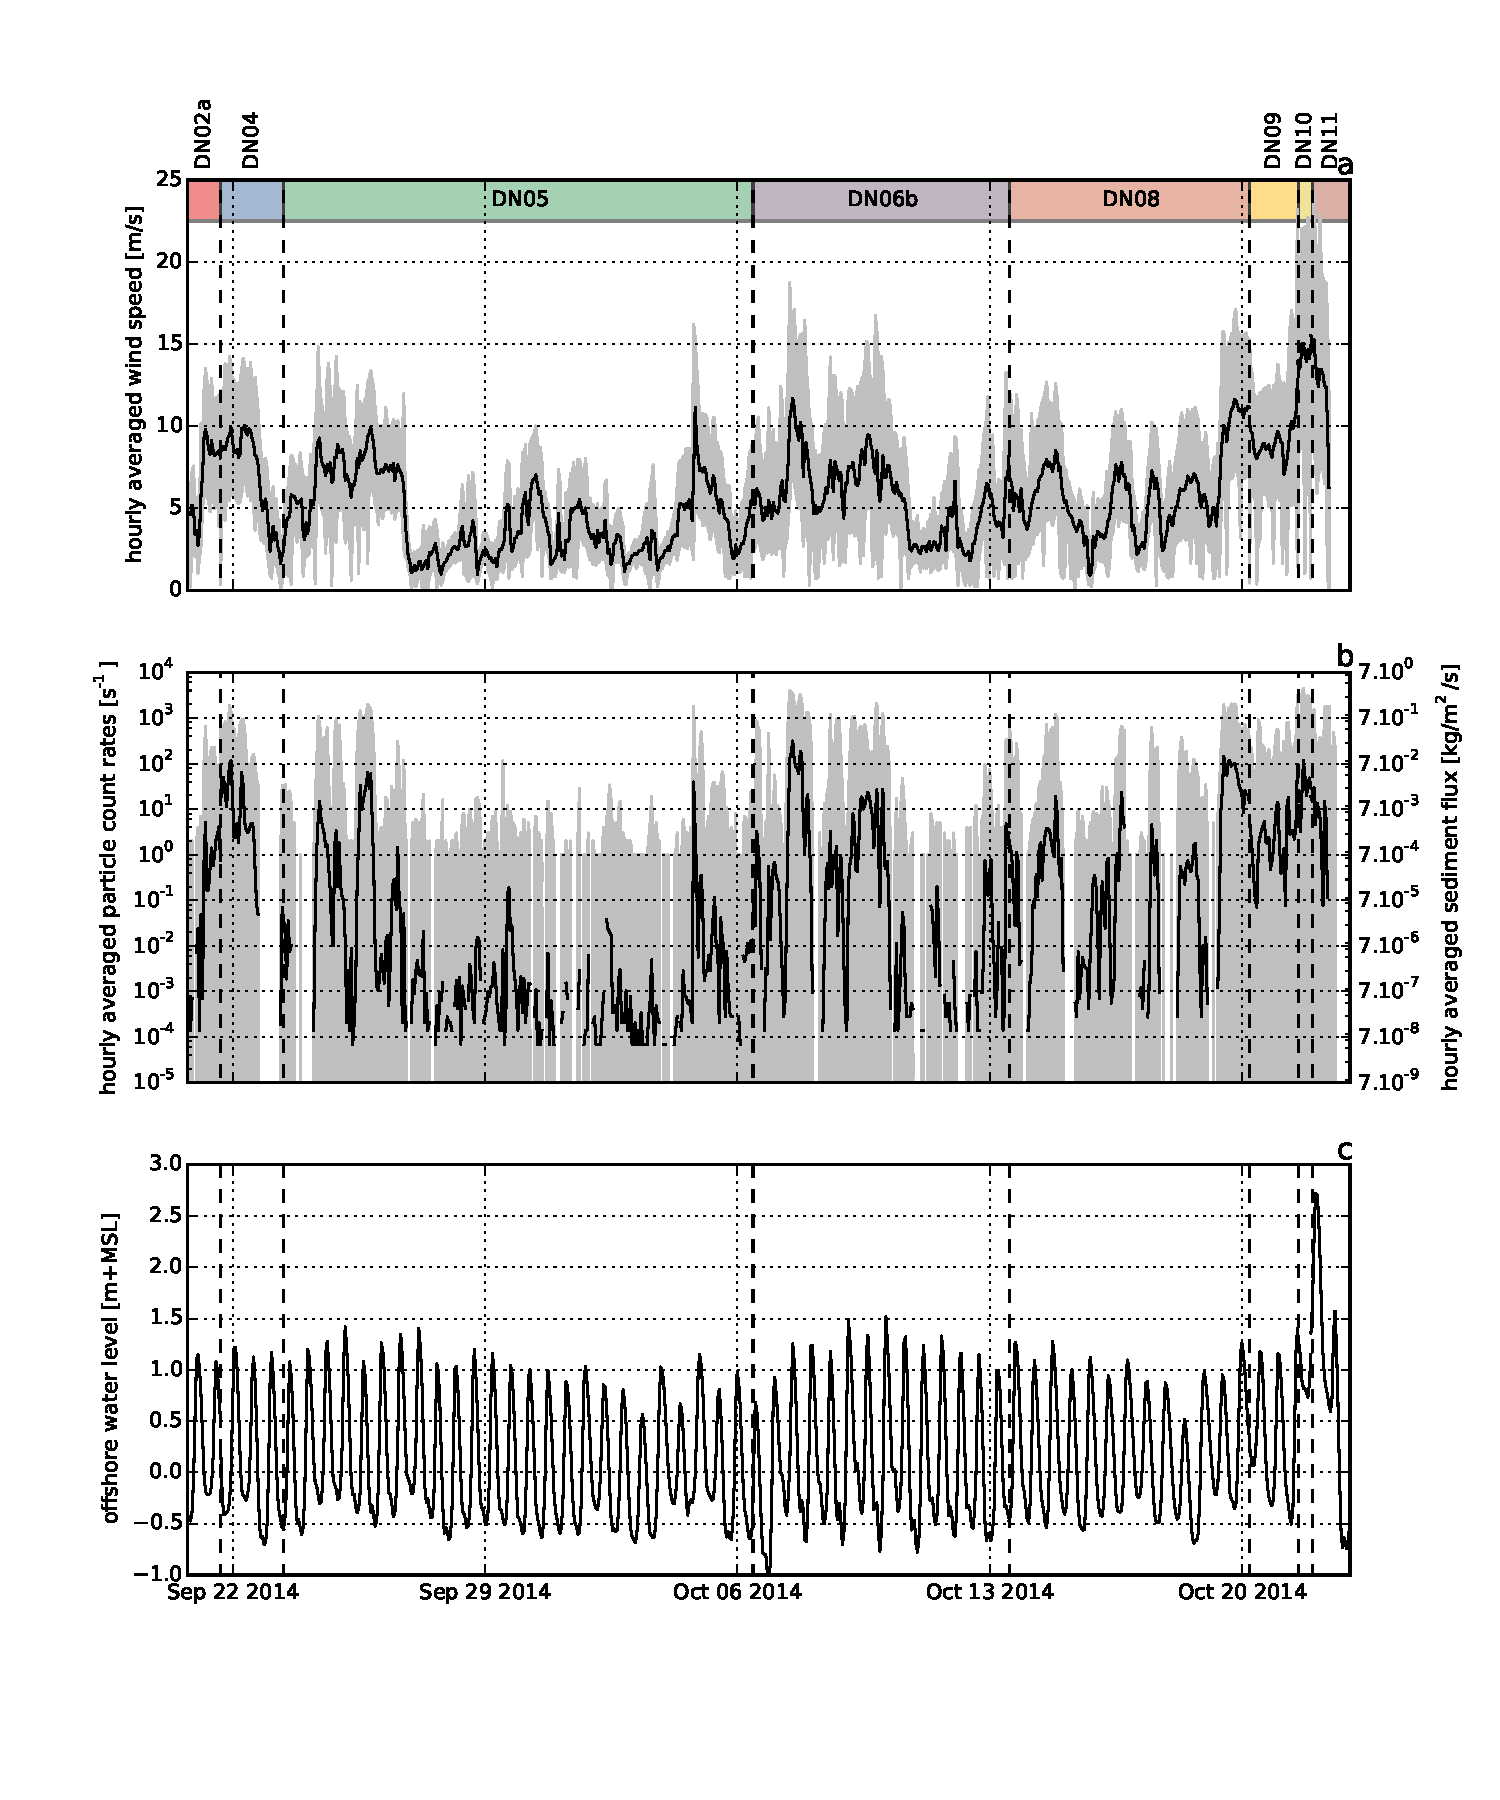
\includegraphics[width=\columnwidth]{../Figures/particlecounts_timeseries}
  \caption{a) Wind time series, b) overall particle count rates during
    the deployments along the westerly transect, and c) offshore tidal
    elevation. Grey lines indicate the raw data, black lines the
    hourly averaged data. Colored bars refer to the deployments listed
    in Table \ref{tab:deployments}. Deployments DN02b and DN06a are
    not included as these are located along different transects.}
  \label{fig:pc_timeseries}
\end{figure}

\begin{figure}
 \centering
  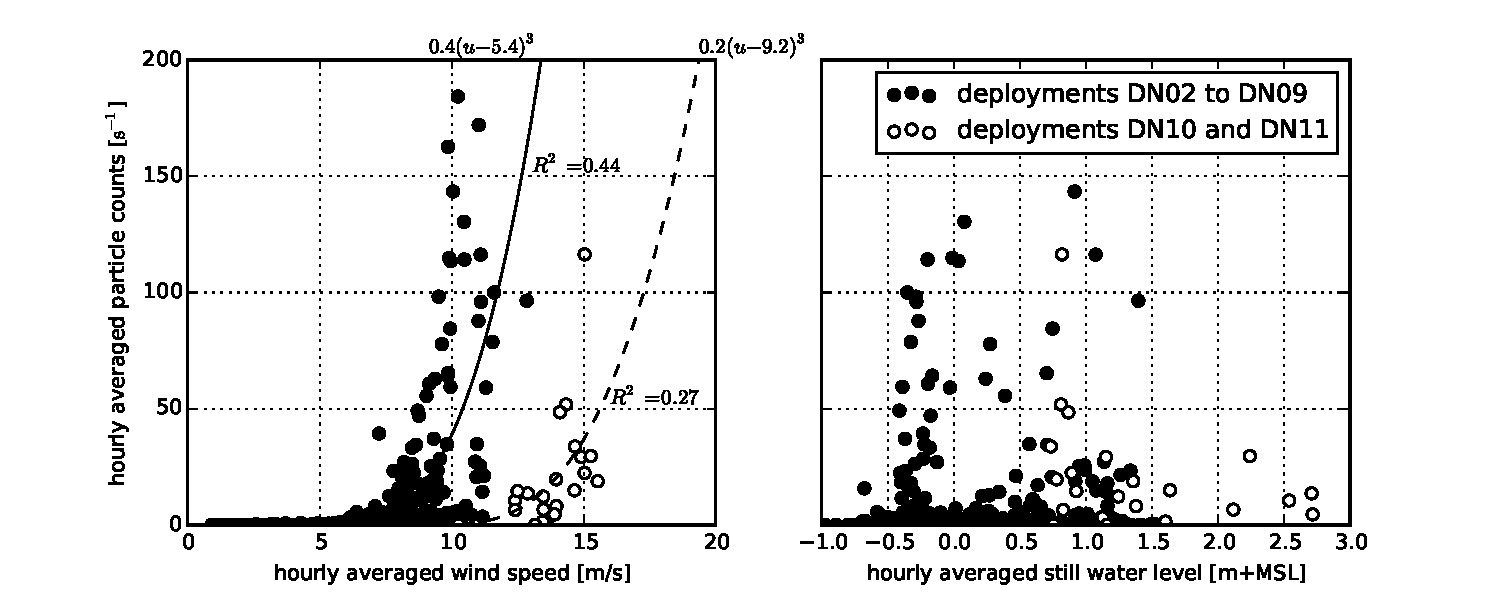
\includegraphics[width=\columnwidth]{../Figures/particlecounts_correlations}
  \caption{a) Relations between overall particle count and wind speed
    or b) water level. Closed circles and continuous lines refer to
    non-storm deployments DN02 to DN09. Open circles and dashed lines
    refer to storm deployments DN10 and DN11. All deployments are
    listed in Table \ref{tab:deployments}.}
  \label{fig:pc_correlations}
\end{figure}

The conditions during the field campaign were characterized by calm
and sunny weather and negligible precipitation, which is unusual for
the time of the year. The average wind speed over the entire
experiment was 6 m/s (Figure \ref{fig:pc_timeseries}a). The maximum
wind speed was registered at 24 m/s at the end of the campaign on
October 23 during the only measured storm event (DN10). The average
overall particle count rate over the entire experiment was 120
$\mathrm{s^{-1}}$ or $< 0.1$ $\mathrm{kg/m^2/s}$ averaged over all
deployed sensors (Figure \ref{fig:pc_timeseries}b). The maximum
overall particle count rate was registered on October 7 at 5800
$\mathrm{s^{-1}}$ or 4 $\mathrm{kg/m^2/s}$ (DN06b). Therefore, the
maximum registered overall particle count rate did not coincide with
the maximum wind speed.

The experiment covered two spring-neap cycles with a tidal range
varying between 1.5 and 2.0 m (Figure \ref{fig:pc_timeseries}c). The
maximum still water level of 2.8 m+MSL was measured during storm
deployment DN11 on October 22. This surge flooded the southern flank
of the Sand Motor up to 5 m+MSL.

\subsection{Relation between sediment transport and wind speed and
  water level}

Periods with low wind conditions seem to coincide with periods with a
negligible overall particle count, whereas periods with fair wind
conditions seem to coincide with periods with a significant overall
particle count (Figure \ref{fig:pc_timeseries}a,b). Also the
occurrence of peaks in overall particle count show a correspondence
with peaks in wind speed. However, the highest peaks in wind speed do
not necessarily coincide with the highest peaks in overall particle
count, resulting in an overall poor correlation between wind speed and
overall particle count (Figure \ref{fig:pc_correlations}a). The poor
correlation is reflected in a Spearman rank correlation coefficient
\citep{Spearman1904} of zero, indicating that the data cannot be
described by a monotonic function of any kind.

In the remainder of this paper it is shown that the storm deployments
DN10 and DN11 provide signals with respect to wind direction, sediment
availability and fetch that are consistently different from the
non-storm deployments DN02 to DN09. In anticipation to these findings,
correlations between wind speed and overall particle count are
computed for the storm and non-storm deployments separately, resulting
in a weak positive relation between wind speed and overall particle
count. Fitting a third-power curve through these separate datasets
results in $R^2$-values of 0.43 and 0.27 respectively. The low
$R^2$-values indicate that much of the variance in the overall
particle count is not explained by wind speed.

No relation between the still water level and the overall particle
count is found (Figure \ref{fig:pc_correlations}b). There is no
evidence that the spring-neap modulation of the high water level of
about 0.5 m influenced the overall particle count significantly.

\subsection{Wind direction and sediment source areas}

\begin{figure}
 \centering
  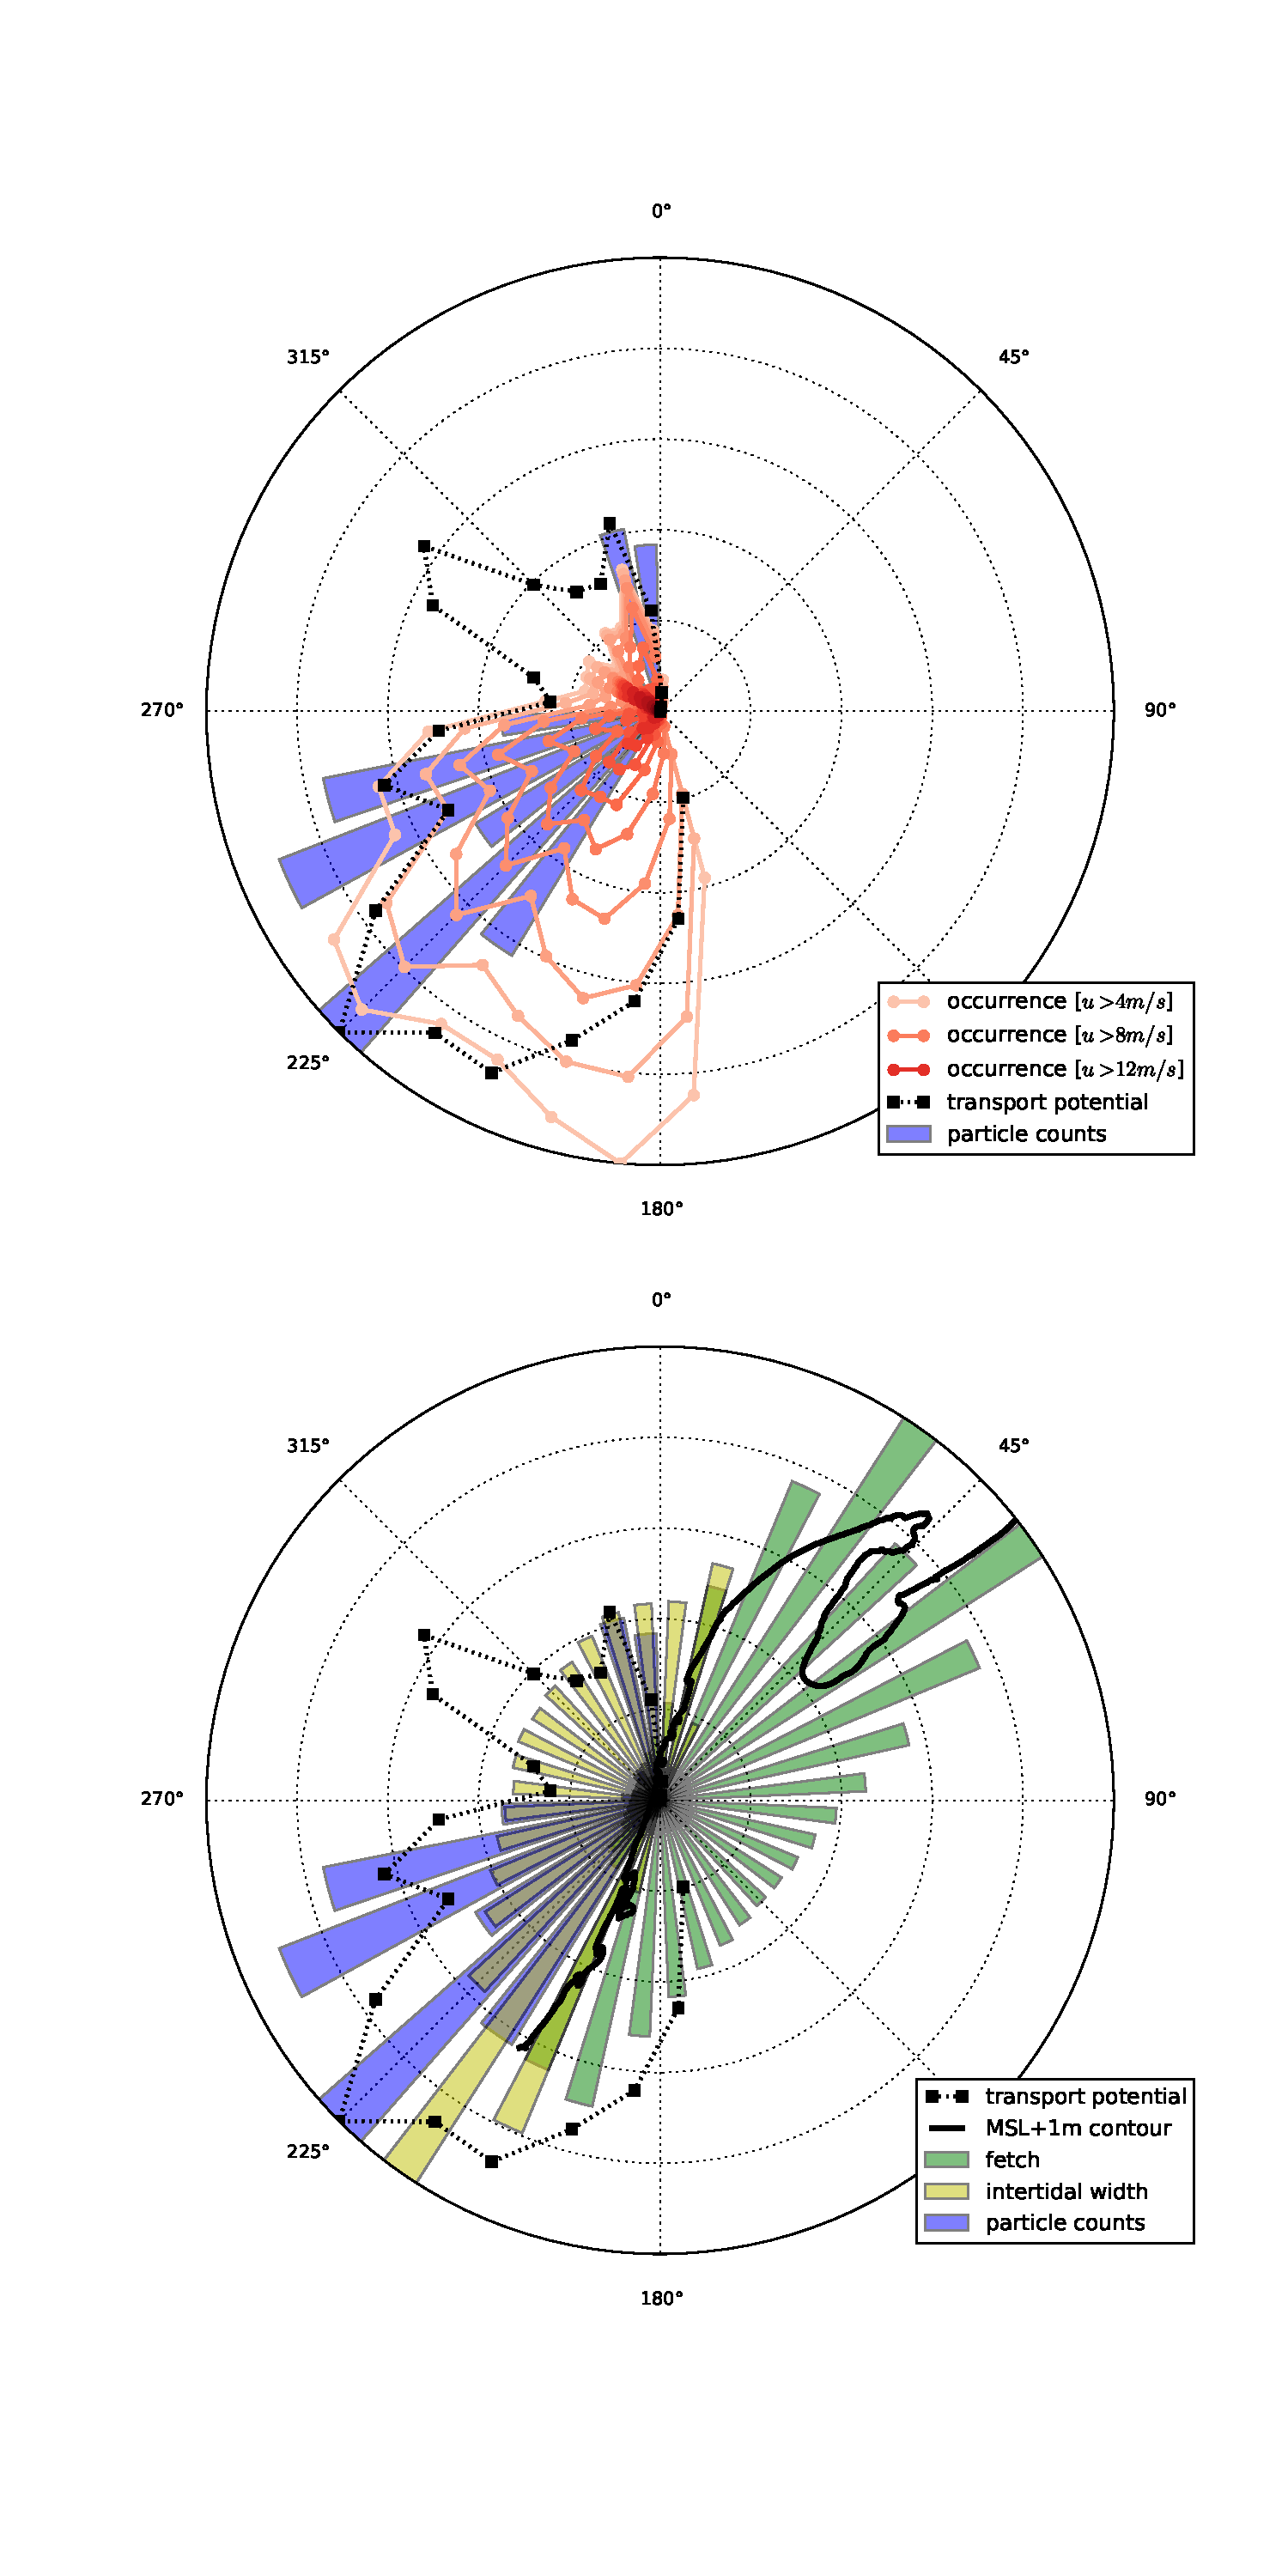
\includegraphics[width=.7\columnwidth]{../Figures/polar_72096_451703}
  \caption{a) Per-mast particle count, wind speed and direction
    obtained from stationary mast (Figure \ref{fig:overview}) and b)
    available fetch and intertidal fetches.}
  \label{fig:pc_direction}
\end{figure}

The vast majority of per-mast particle counts registered at the
stationary mast, that was located at the high water line during almost
the entire field campaign (Figure \ref{fig:overview}), was registered
from a limited number of wind directions. These directions do not
coincide with the prevailing wind direction or the wind direction with
the largest transport potential (Figure \ref{fig:pc_direction}a).

Figure \ref{fig:pc_direction}a shows that the prevailing wind
direction was south, but that the largest transport potential
(Equation \ref{eq:transport_potential}) came from the southwesterly
and northwesterly directions. The per-mast particle count does not
align with the prevailing wind direction or the directions with the
largest transport potential as both the southerly and northwesterly
wind directions did not induce a significant particle count.

Figure \ref{fig:pc_direction}b shows that most particles are
registered from the wind directions with the shortest
fetches. However, these wind directions provide among the largest
intertidal beach widths along the Dutch coast. The exception is the
northwesterly wind direction, that does accommodate a fair intertidal
beach width, but did not register a per-mast particle count close to
what could be expected from the transport potential. The northwesterly
wind directions were solely present during the storm deployment DN10.

\subsection{Spatial gradients in sediment transport}

\begin{figure}
 \centering
  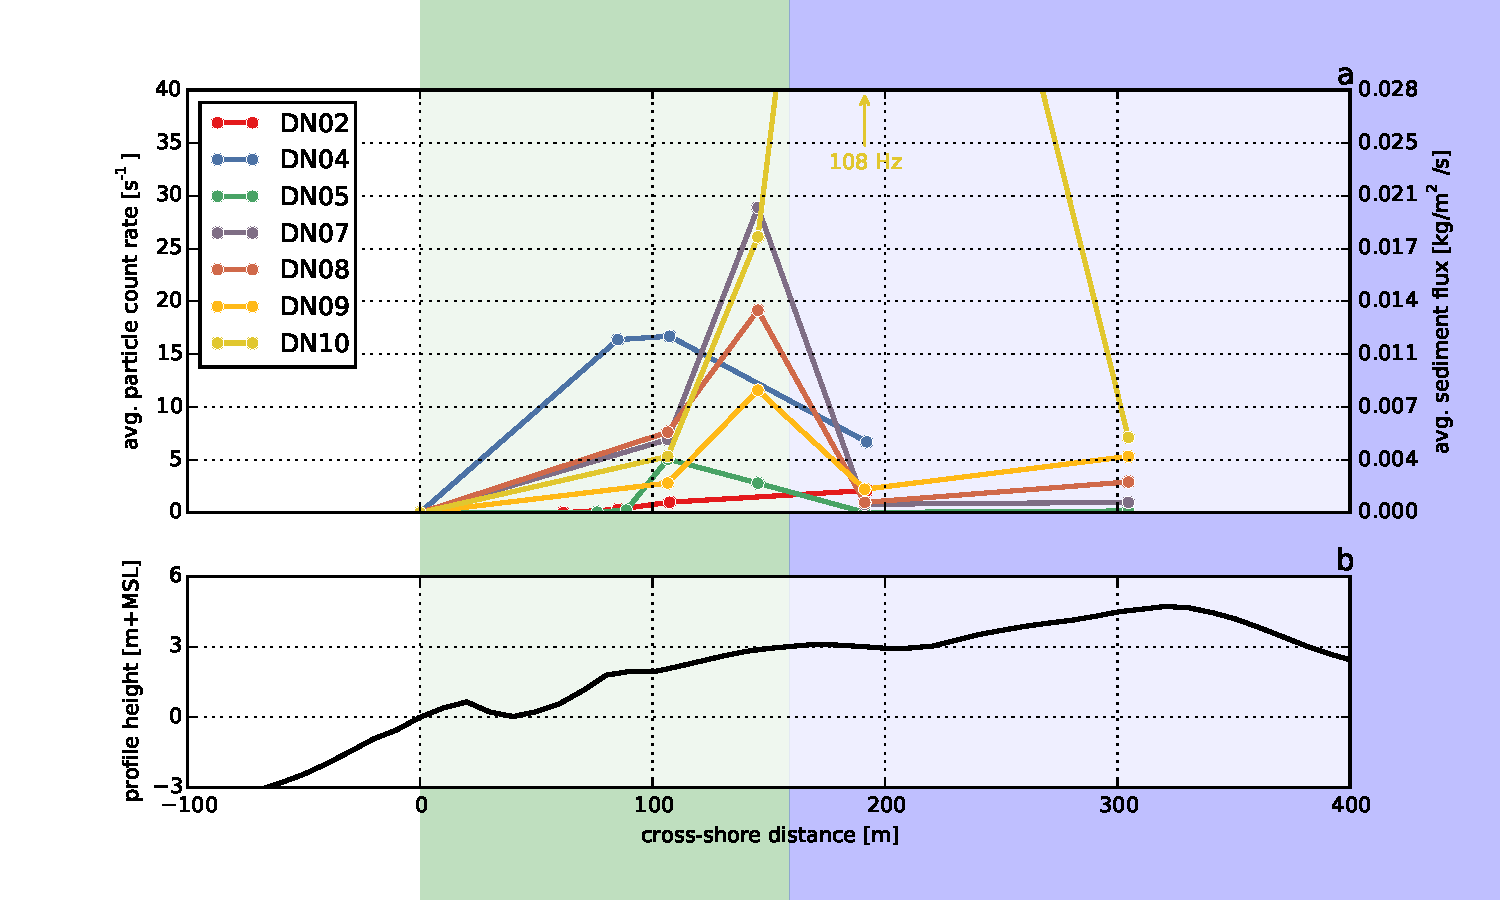
\includegraphics[width=\columnwidth]{../Figures/particlecounts_transects}
  \caption{a) Average per-mast particle count rates during the
    deployments along the westerly transect and b) beach profile at
    the beginning of the field campaign. Line colors refer to the
    partitioning of the time series in Figure
    \ref{fig:pc_timeseries}.}
  \label{fig:pc_transect}
\end{figure}

\begin{figure}
 \centering
  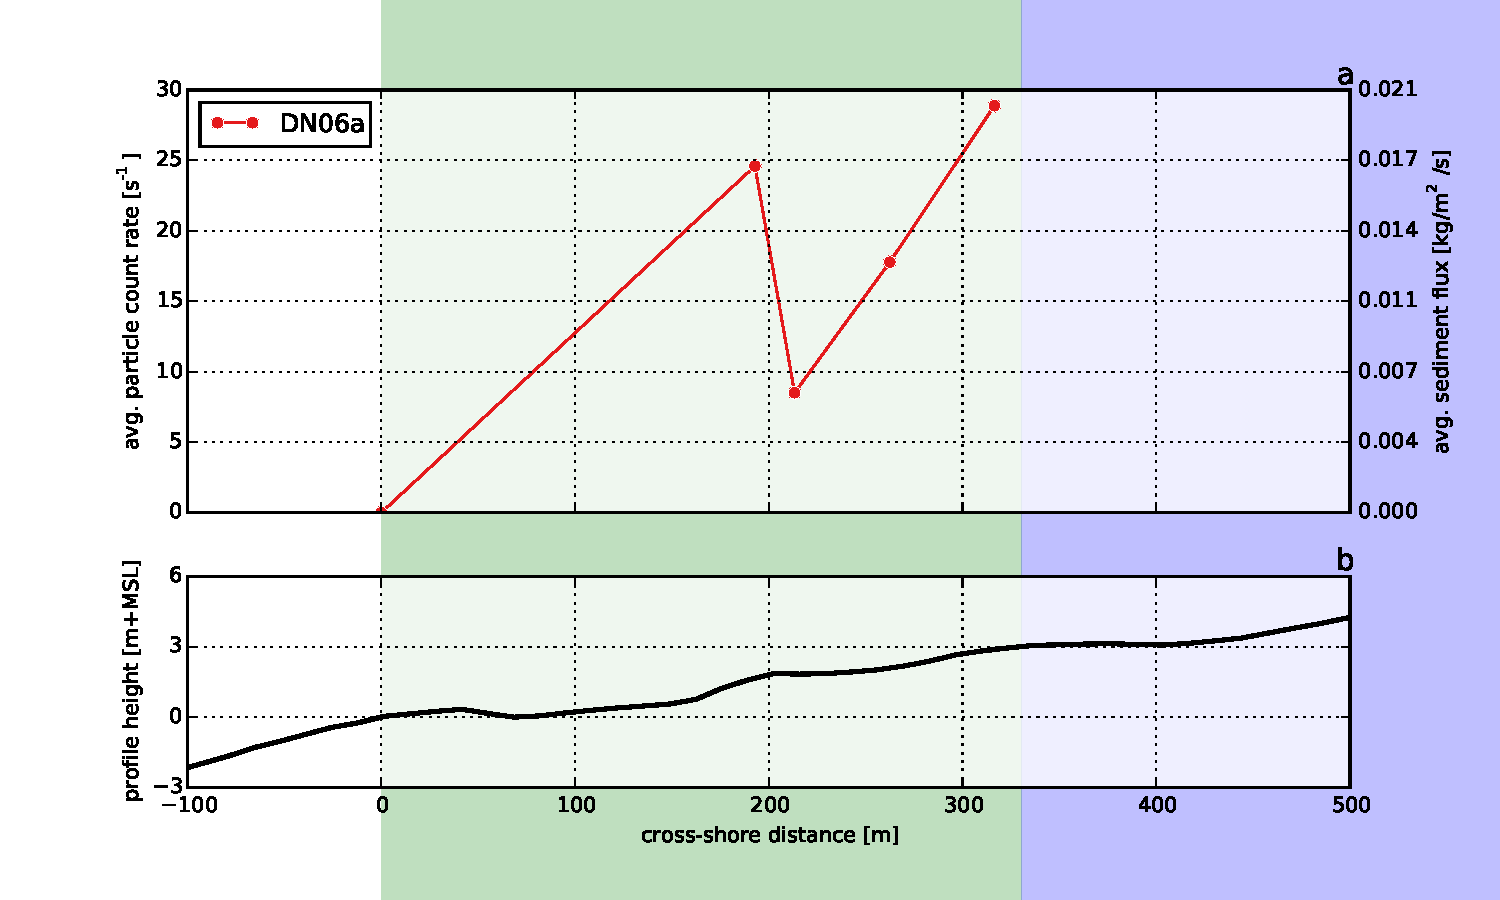
\includegraphics[width=\columnwidth]{../Figures/particlecounts_DN06}
  \caption{a) Average per-mast particle count rates during deployment
    DN06a along the southwesterly transect and b) beach profile at the
    beginning of deployment DN06.}
  \label{fig:pc_transect_DN06}
\end{figure}

\begin{figure}
 \centering
  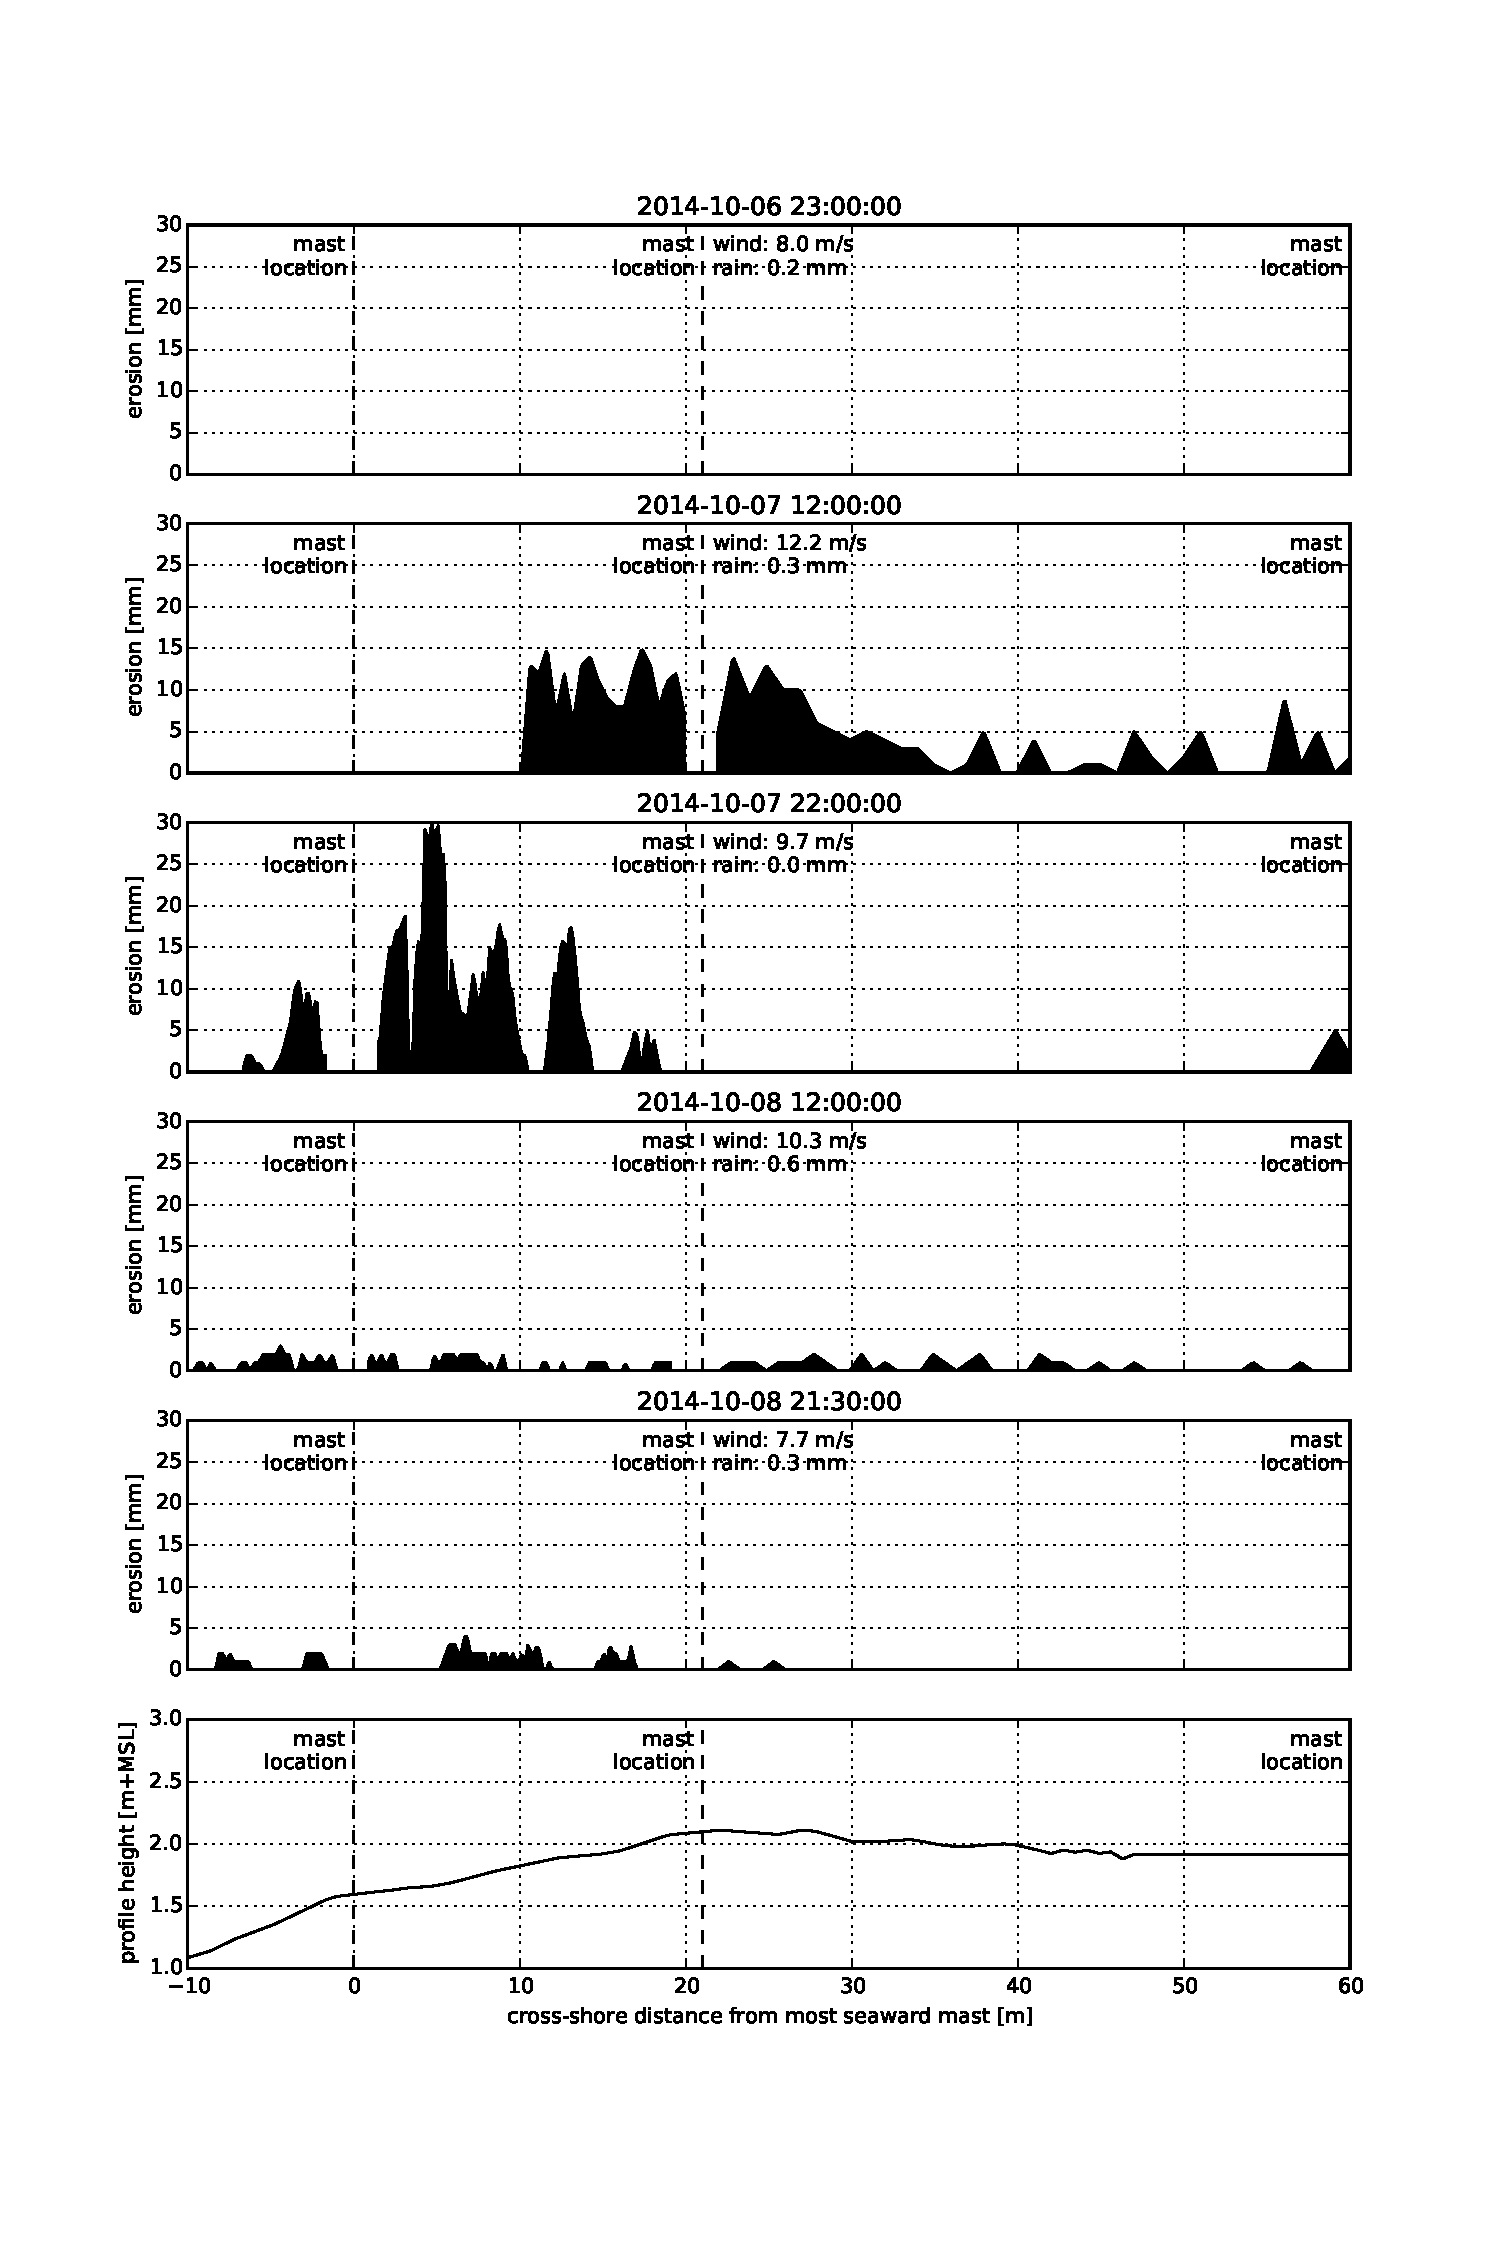
\includegraphics[width=\columnwidth]{../Figures/nails}
  \caption{Erosion measured using erosion pins during five tidal
    cycles during deployment DN06a along the southwesterly transect.}
  \label{fig:nails}
\end{figure}

Significant variations in per-mast particle count along the
measurement transects is found. Figure \ref{fig:pc_transect} shows
that the largest increase in per-mast particle count in downwind
direction (positive gradients) is consistently located in the
intertidal beach area. Positive gradients in sediment transport
indicate a net erosion of the beach surface and thus entrainment of
sediment.
% The positive gradients in the intertidal beach area therefore suggest
% that the intertidal beach is an important source of aeolian
% sediment. The small positive gradients over the dry beach similarly
% suggest that this area is a minor source of sediment.

A significant decrease in per-mast particle count in downwind
direction (negative gradients) is consistently found at the transition
between intertidal and dry beach. Negative gradients in sediment
transport indicate net deposition of sediment. Only during storm
deployment DN10 the negative gradients at the transition were absent
and large positive gradients in both the intertidal and dry beach area
were found (Figure \ref{fig:pc_transect}).
% The negative gradients therefore indicate that deposition of sediment
% occurs locally at the transition between intertidal and dry beach.

The negative gradients coincide with the transition from the berm
slope to the berm flat. Local deposition of aeolian sediment at the
edge of a berm appears to be consistent behavior as it is also
observed within the intertidal beach area. Four masts were deployed
along a southwesterly transect within the intertidal beach area
(DN06a, Figure \ref{fig:pc_transect_DN06}) concurrent with deployment
DN06b. These measurements show a significant decrease in per-mast
particle count over a minor berm-like feature (x = 200 m) in the
intertidal beach area. Downwind of this feature the per-mast particle
count increased again with a rate comparable to what was found upwind
of the berm-like feature. In addition, small scale measurements on bed
level change confirm that erosion by wind is concentrated on the berm
slope (Figure \ref{fig:nails}), while the berm flat tends to
accrete. The maximum erosion of 1.2 cm in a single tidal cycle was
measured with wind speeds above 10 m/s and little precipitation.

\begin{figure}
 \centering
  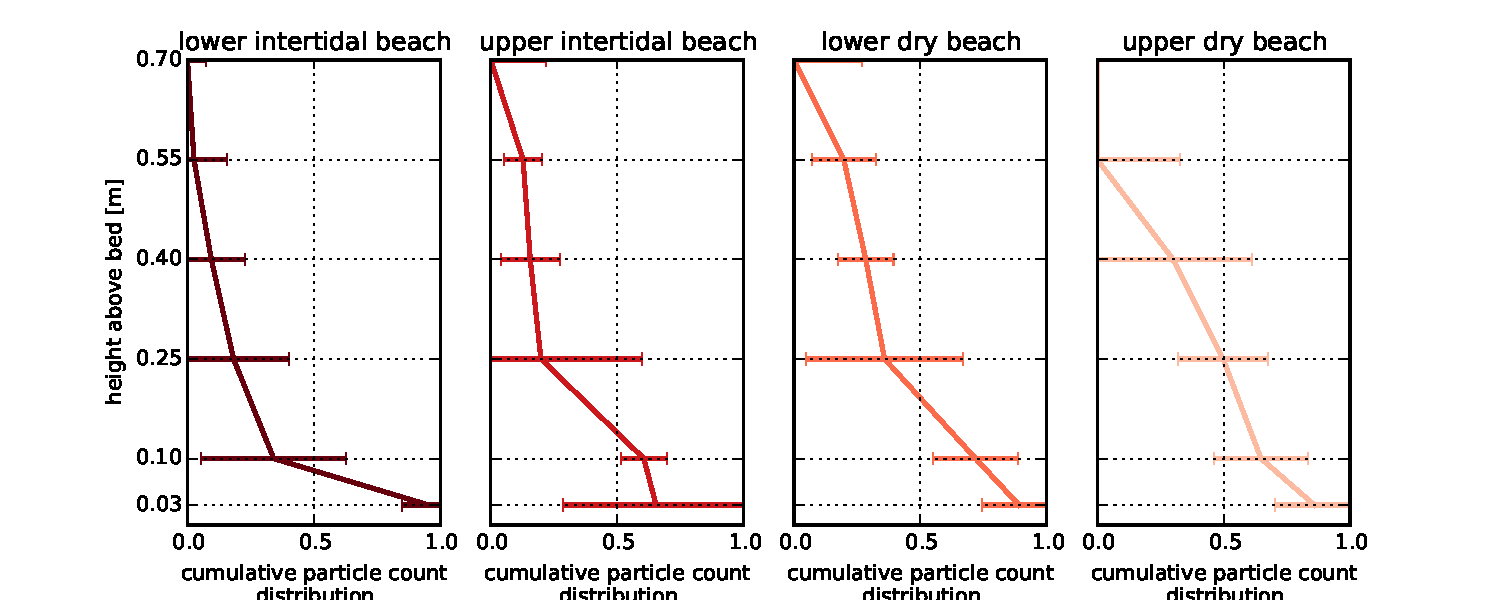
\includegraphics[width=\columnwidth]{../Figures/particlecounts_distheight}
  \caption{Cumulative particle count distribution over the vertical
    during deployment DN08. The line indicates the percentage of
    particles that bypasses a certain height above the bed. The
    horizontal bars visualize the variability in time of the particle
    count per laser sensor.}
  \label{fig:pc_distheight}
\end{figure}

Measured negative gradients might also be caused by sediment locally
bypassing the measurement equipment. To ensure that the number of
bypassing particles is limited, the most landward mast in each
transect was permanently equipped with six laser sensors up to 70 cm
above the bed. The number of particles counted in the upper laser
sensor was consistently low ($\leq 1\%$), suggesting that only a small
number of particles bypassed the equipment at this point.

At the location downwind of the negative gradients more sediment might
have bypassed than at the most landward measurement location. During
deployment DN08 all four masts were equipped with six laser sensors in
order to capture the vertical distribution of the particle count
across the beach (Figure \ref{fig:pc_distheight}). It appears that the
center of gravity of the particle count moves upward in downwind
direction.%, which seems in accordance with the development of a
%boundary layer
Downwind of the negative transport gradient the
percentage of particles counted by the upper laser sensor is 20\%
compared to $\leq 10\%$ at the other locations, suggesting that most
particles bypassed at this location. The difference between the
fraction of bypassing particles is too small to explain the large
negative gradients, but are likely to cause the measured negative
gradients to be overestimated.

\subsection{Fetch vs. sediment availability}

\begin{figure}
 \centering
  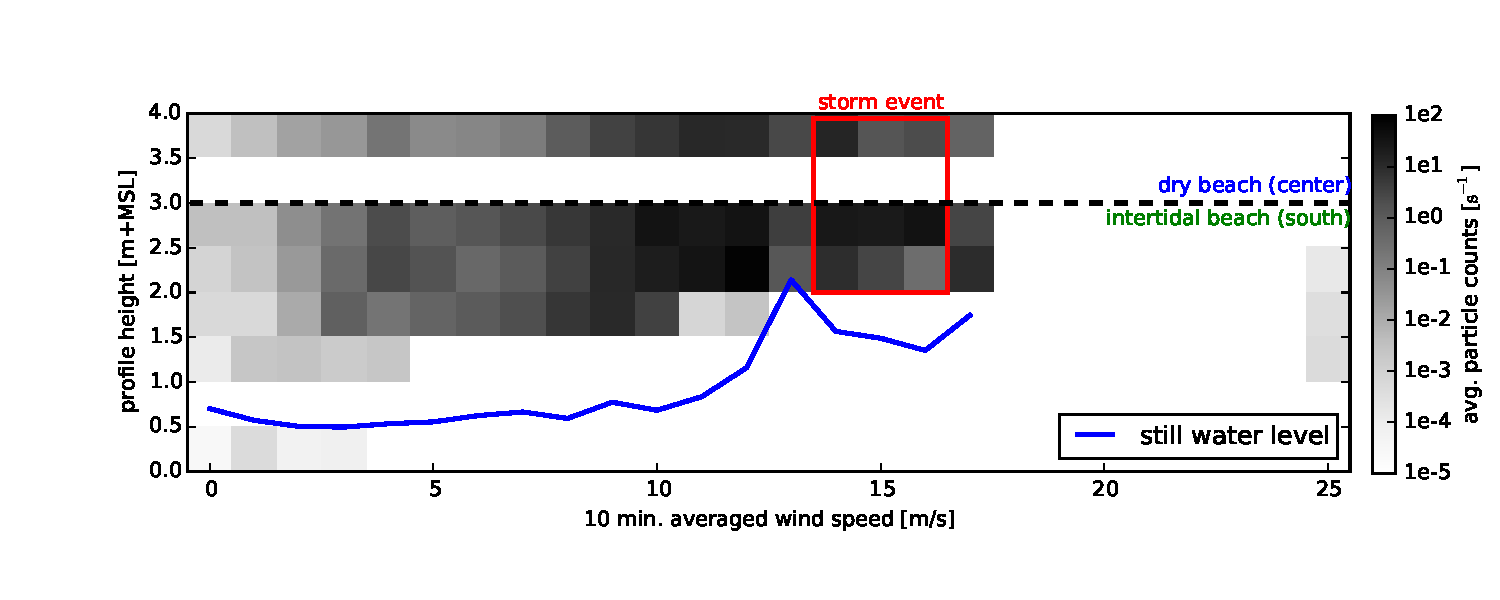
\includegraphics[width=\columnwidth]{../Figures/particlecounts_velocities}
  \caption{Average overall particle count rates depending on governing
    wind speed and bed level at measurement location, and average
    still water level depending on governing wind speed.}
  \label{fig:pc_velocity}
\end{figure}

In Figure \ref{fig:pc_velocity} the overall particle count obtained
during the field campaign is binned according to the prevailing wind
speed and the bed level at the measurement location. The average still
water level is an indication of available fetch. The peak in overall
particle count is at 3 m+MSL irrespective of the wind speed and
available fetch. Therefore the overall particle count seems to be
limited by location rather than wind speed or available fetch. The
specific location at which the particle count peaks corresponds to the
high water line and the onset of the shell pavement that largely
covers the dry beach.

\section{Discussion}

% positive gradients
The positive gradients in per-mast particle count in the intertidal
beach area and minor positive gradients in the dry beach area suggest
that the intertidal beach is a primary source of aeolian sediment in
the Sand Motor region. This observation is in accordance with the
large scale sediment budgets of the Sand Motor region
\citep{Hoonhout2017a}. Armoring of the dry beach surface, due to
formation of lag deposits, might lead to a significant reduction in
local aeolian sediment availability. Similarly, sediment availability
might also be limited in the intertidal beach area due to periodic
flooding and consequently high soil moisture contents. From the
differences in per-mast particle count gradients between the
intertidal and dry beach it can be assumed that the reduction of
sediment availability due to armoring outweighs the influence of soil
moisture. Local differences in bed surface properties would therefore
induce relative differences in sediment availability that govern
aeolian sediment transport in the Sand Motor region.

\begin{figure}
  \centering
  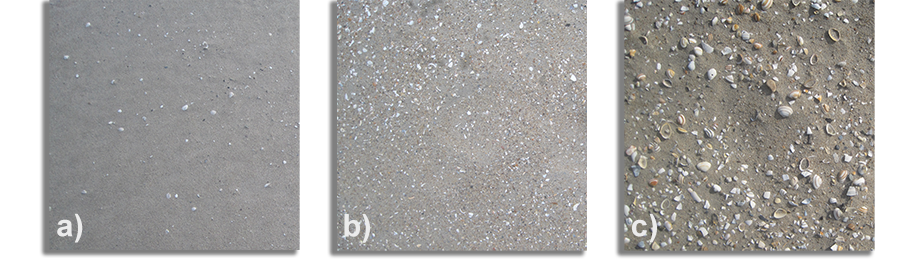
\includegraphics[width=\columnwidth]{../Figures/armoring_small}
  \caption{Visual impression of armor layer at three locations in the
    Sand Motor region: a) intertidal beach, no armoring b) lower dry
    beach, minor armoring with shell fragments c) upper dry beach,
    severe armoring with many shells and coarse sand. Covered surface
    is approximately 40 x 40 cm in all cases.}
  \label{fig:armoring}
\end{figure}

% negative gradients
The negative gradients in per-mast particle count at the transition
between intertidal and dry beach indicate that sediment eroded from
the intertidal beach is deposited locally on the dry
beach. Morphological feedback with the wind might cause the sediment
transport capacity to peak at the berm edge due to the presence of a
locally accelerated wind \citep[i.e. jet flow;][]{Hesp2016}, resulting
in deposition at the berm flat. In addition, the berm edge coincides
with the visually observed onset of a shell pavement (Figure
\ref{fig:armoring}). The shell pavement emerged from the nourished
sediment in the first half year after construction of the Sand Motor
\citep{Hoonhout2017a} due to winnowing of sand from the bed. Roughness
elements, like shells and cobbles, might trap impacting grains, and
hamper saltation, or cause fully elastic collisions, and enhance
saltation. The shell pavement at the measurement locations is
relatively open and therefore both processes are likely to be
relevant. The consistent negative gradients in particle count at the
onset of the shell pavement suggest that trapping of sediment is
dominant over the enhancement of saltation due to fully elastic
collisions.

% local storage and correlation water levels
\begin{figure}
 \centering
  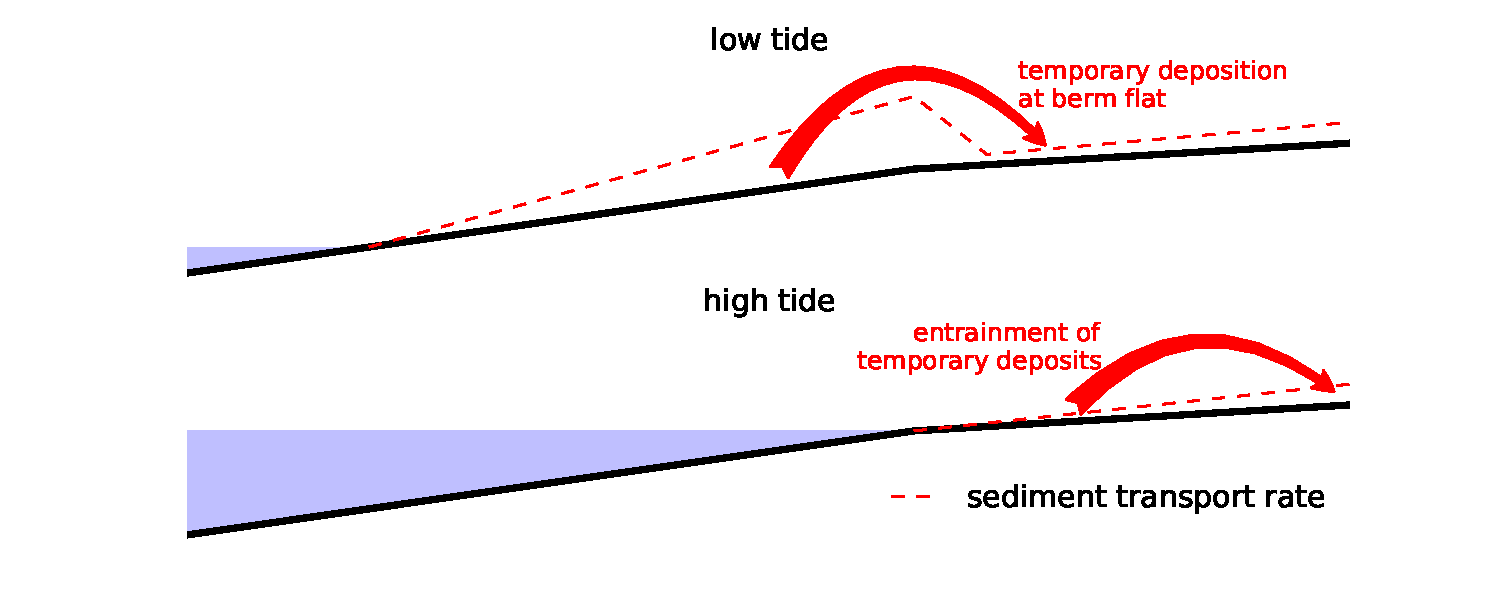
\includegraphics[width=\columnwidth]{../Figures/temporal_deposits}
  \caption{Conceptual illustration of how temporal deposits facilitate
    a continuous sediment supply from the intertidal beach to the
    dunes.}
  \label{fig:temporal_deposits}
\end{figure}

The local deposition of sediment at the berm flat is temporary as no
accumulation of sand is observed on top of the shell pavement during
the \textsc{MegaPEX} field campaign. This suggests that sediment
supply from marine sources and deposition in dunes, dune lake and
lagoon is a phased process. In a phased system the local sediment
deposits at the berm flat might act as temporary sediment source
during high water (Figure \ref{fig:temporal_deposits}). Consequently,
measured aeolian sediment transport rates would be continuous and
independent of the instantaneous water level. The phasing of erosion
and deposition can therefore explain the weak correlations between
measured overall particle count and the instantaneous water level,
which seemed to contrast the conclusion that the intertidal beach is a
primary source of aeolian sediment.

The phasing of erosion and deposition increases the duration of
transport from the intertidal beach to the dunes. The environmental
conditions therefore needs to be favorable for aeolian sediment
transport over a longer period for the sediment to reach the
dunes. This requirement for dune growth closely relates to the need
for synchronization between sediment availability and wind transport
capacity emphasized by \citet{Houser2009, Anthony2013}.

% water level
%Low average water levels accommodate initiation of aeolian sediment
%transport relatively distant from the high water line where the
%overall particle count tends to peak. As average water levels increase
%with increasing wind speed, due to wind setup, the available fetch
%decreases. Nevertheless, the overall particle count still peaks close
%to the high water line and not beyond. Moreover, the height of the
%peak in overall particle count increases with increasing wind
%speed. Both the decrease in available fetch and the increase in
%maximum overall particle count result in an increase in overall
%particle count gradient over the intertidal beach.  The increased
%gradient indicates that also the rate of sediment entrainment in the
%intertidal beach area increases and overcompensates the decrease in
%fetch. Also the entrainment rate at the dry beach increases with
%increasing wind speed, but to a significantly less extent than at the
%intertidal beach. The exception is again the storm deployment DN10,
%which shows a peak in overall particle count landward of the high
%water line.

% high wind events
%The per-mast particle count obtained during the storm deployment DN10
%appeared to be exceptional with respect to the other non-storm
%deployments: the overall particle count during deployment DN10 was low
%compared to the prevailing wind speed and direction, the negative
%gradients in per-mast particle count at the transition between
%intertidal and dry beach were absent and the peak in overall particle
%count did not coincide with the high water line or berm edge.

During a high wind event the relative importance of limitations in
sediment availability might change. Strong winds can mobilize even the
largest sediment fractions and shell fragments. Consequently, the
beach armor layer itself might be transported and its reducing effect
on sediment availability might be (partially) neutralized. Also the
trapping of sediment due to an increase in bed roughness might be less
effective and the influence of the berm on the wind flow reduced. In
addition, high wind events are regularly accompanied with surges that
prevent erosion of the intertidal beach by wind. Instead, the wind
energy can be used for erosion of the dry beach, which contributes to
the removal of the beach armor layer. The surge itself might also
remove the beach armor layer by wave action or bury it by deposition
of marine sediments. The removal or burial of the beach armor layer
might elevate sediment availability from the dry beach also after the
the storm passed. Only after development of a new beach armor layer
the sediment availability and transport rates then equal the pre-storm
situation.

The significant spatial variations in sediment transport gradients
reflect significant variations in aeolian sediment availability. The
formation of beach armor layers is known to limit aeolian sediment
availability \citep{McKennaNeuman2012} and cause spatial variations in
aeolian sediment supply \citep{Jackson2010}. In case of the Sand Motor
the formation of the beach armor layer is particularly accommodated
by:
\begin{enumerate}
\item the high number of shells and other roughness elements that is
  generally contained by nourishment sand \citep{VanDerWal1998,
    VanDerWal2000}, and
\item the high construction height of the Sand Motor.
\end{enumerate}
As the majority of the Sand Motor's subaerial surface has never been
influenced by hydrodynamics, the beach surface in these areas is never
reworked. Consequently, the majority of the Sand Motor's subaerial
surface does not directly contribute to dune growth or beach-dune
interactions \citep{Houser2013}. The vast beach surface seems to
stimulate dune growth only indirectly by sheltering the dunes from
storm erosion.

Large scale nourishments are typically presented as natural solution
to improve coastal safety. The natural dynamics of beach-dune systems
depend on the periodic reworking of the beach surface as it prevents
the formation of lag deposits. Large scale nourishments with a
construction height above regular storm level can disrupt these
natural dynamics as the formation of lag deposits is accommodated. The
resulting compartmentalization of the beach can result in a phased
process that decelerates dune growth and make dune growth more
dependent on incidental storm events. Besides, also marine erosion
would likely be limited, contributing to the lifetime of the
nourishment.  In contrast, limiting the construction height of large
scale nourishments would reduce the lifetime of a nourishment, but
result in a larger source area of aeolian sediment and the stimulation
of dune growth and natural beach-dune interactions.

\section{Conclusions}

The Sand Motor (or Sand Engine) is a 21 $\mathrm{Mm^3}$ mega
nourishment along the Dutch coast that is constructed well above storm
surge level \citep{Stive2013} and therefore largely shaped by
wind. During the six week \textsc{MegaPeX} field campaign in the fall
of 2014, spatial gradients in aeolian sediment transport were
measured. The gradients identified the intertidal beach as the primary
source of aeolian sediment. In addition, local temporal deposition of
sediment at the berm flat occurred. The deposition is likely caused by
a combination of morphological feedback with the wind and an increase
in bed roughness due to the presence of a shell pavement. The local
deposition of sediment causes the transport of sediment from
intertidal beach to dunes, dune lake and lagoon to be phased.

\bigskip

\noindent From the measurements the following conclusions can be drawn:

\begin{enumerate}
\item In the Sand Motor region, the (southern) intertidal beach area
  is a more important source of aeolian sediment than the dry beach
  area.
\item The relative importance of the intertidal beach as supplier of
  aeolian sediment could be explained by the development of a beach
  armor layer in the dry beach area that outweighs the influence of
  high soil moisture contents in the intertidal beach area.
\item Aeolian sediment originating from the intertidal beach seems to
  settle on the berm flat and to be gradually transported further
  resulting in an continuous sediment flux from the intertidal beach
  area and into the dunes, even if the intertidal beach is flooded.
\item During high wind events, aeolian sediment availability in the
  intertidal beach area tends to be reduced by high water levels,
  while the sediment availability in the dry beach area tends to be
  increased due to mobilization of the beach armor layer;
\item The construction height of a mega nourishment is important to
  its lifetime as it is governs compartmentalization of the beach due
  to beach armoring.
\end{enumerate}

%%% Local Variables:
%%% mode: latex
%%% TeX-master: "./thesis"
%%% End:
